\documentclass[tikz]{standalone}
\usepackage{tikz}
\usetikzlibrary{backgrounds,matrix,positioning}

\begin{document}
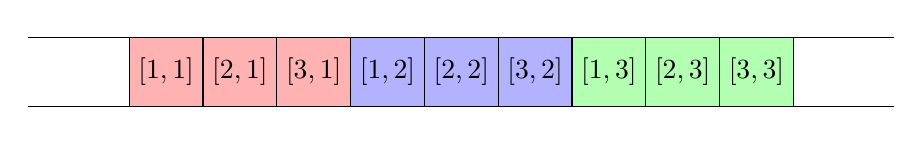
\begin{tikzpicture}[
    arraynode/.style={
        draw,
        rectangle,
        minimum size = 25pt,
        anchor = center,
        },
    array/.style={
        matrix of math nodes,
        nodes = arraynode,
        row sep = -\pgflinewidth,
        column sep = -\pgflinewidth,
        % column sep = 0pt,
        % row sep = 0pt,
        nodes in empty cells,
        column 1/.style={nodes={fill=red!30}},
        column 2/.style={nodes={fill=red!30}},
        column 3/.style={nodes={fill=red!30}},
        column 4/.style={nodes={fill=blue!30}},
        column 5/.style={nodes={fill=blue!30}},
        column 6/.style={nodes={fill=blue!30}},
        column 7/.style={nodes={fill=green!30}},
        column 8/.style={nodes={fill=green!30}},
        column 9/.style={nodes={fill=green!30}},
        },
]

\draw[black] (-5.5,+12.5pt) -- (+5.5,+12.5pt);
\draw[black] (-5.5,-12.5pt) -- (+5.5,-12.5pt);

\matrix [array] {
    {[1,1]} & {[2,1]} & {[3,1]} & {[1,2]} & {[2,2]} & {[3,2]} & {[1,3]} & {[2,3]} & {[3,3]} \\
};

\end{tikzpicture}%
\end{document}